% ============================================================
%  Verifiable Smart Contract Deployer — Project Report
%  Overleaf / pdfLaTeX  |  ~5-6 pages
% ============================================================
\documentclass[11pt,a4paper]{article}

\usepackage[T1]{fontenc}
\usepackage[utf8]{inputenc}
\usepackage[margin=2.2cm]{geometry}
\usepackage{lmodern}
\usepackage{microtype}
\usepackage{parskip}
\usepackage{titlesec}
\usepackage{fancyhdr}
\usepackage{booktabs}
\usepackage{tabularx}
\usepackage{enumitem}
\usepackage{listings}
\usepackage{xcolor}
\usepackage{hyperref}
\usepackage{float}
\usepackage{tikz}
\usepackage{tcolorbox}
\usetikzlibrary{shapes.geometric,arrows.meta,positioning}
\tcbuselibrary{skins}

% ── Colours ─────────────────────────────────────────────────
\definecolor{codeblue}{rgb}{0.09,0.39,0.69}
\definecolor{codegreen}{rgb}{0.13,0.55,0.13}
\definecolor{codegray}{rgb}{0.5,0.5,0.5}
\definecolor{codepurple}{rgb}{0.38,0.15,0.69}
\definecolor{backcolour}{rgb}{0.97,0.97,0.97}
\definecolor{accentcyan}{RGB}{6,182,212}
\definecolor{accentpurple}{RGB}{124,92,191}

% ── Code style ───────────────────────────────────────────────
\lstset{
  backgroundcolor=\color{backcolour},
  basicstyle=\ttfamily\scriptsize,
  keywordstyle=\color{codeblue}\bfseries,
  commentstyle=\color{codegreen}\itshape,
  stringstyle=\color{codepurple},
  numberstyle=\tiny\color{codegray},
  breaklines=true, numbers=left, numbersep=4pt,
  frame=single, framesep=2pt, rulecolor=\color{gray!40},
  tabsize=2, captionpos=b,
}
\lstdefinelanguage{Solidity}{
  keywords={pragma,solidity,contract,function,returns,mapping,address,
            uint256,bytes32,string,bool,struct,event,emit,constructor,
            public,external,view,memory,calldata,require,delete},
  keywordstyle=\color{codeblue}\bfseries,
  comment=[l]{//}, morecomment=[s]{/*}{*/},
  commentstyle=\color{codegreen}\itshape,
  sensitive=true,
}

% ── Section style ────────────────────────────────────────────
\titleformat{\section}{\large\bfseries}{}{0em}{}[\color{accentcyan}\titlerule]
\titleformat{\subsection}{\normalsize\bfseries}{}{0em}{}
\titlespacing{\section}{0pt}{10pt}{4pt}
\titlespacing{\subsection}{0pt}{6pt}{2pt}

% ── Header / footer ─────────────────────────────────────────
\pagestyle{fancy}\fancyhf{}
\fancyhead[L]{\small\textcolor{gray}{Verifiable Smart Contract Deployer}}
\fancyhead[R]{\small\textcolor{gray}{Project Report}}
\fancyfoot[C]{\thepage}
\renewcommand{\headrulewidth}{0.4pt}

\hypersetup{colorlinks,linkcolor=accentpurple,urlcolor=accentcyan,
            pdftitle={Verifiable Smart Contract Deployer}}

% ── Title ────────────────────────────────────────────────────
\title{\vspace{-1.5em}\textbf{Verifiable Smart Contract Deployer}\\[0.3em]
       \large A Cryptographic Security Gate for Sepolia Deployments}
\author{Project Report}
\date{\today}

% ============================================================
\begin{document}
% ============================================================
\maketitle\thispagestyle{fancy}\vspace{-1em}

% ── Abstract ────────────────────────────────────────────────
\begin{tcolorbox}[colback=accentcyan!6,colframe=accentcyan!50,
                  fonttitle=\bfseries,title=Abstract,left=4pt,right=4pt,top=3pt,bottom=3pt]
\small
The \textbf{Verifiable Smart Contract Deployer} is a full-stack security gate that enforces
cryptographic trust in Ethereum Sepolia smart contract deployments through a four-factor
pipeline: SHA-256 artifact hashing, auditor pre-approval, keyless Sigstore/Cosign verification,
and on-chain runtime bytecode matching via \texttt{eth\_getCode}. Only deployments passing all
four checks atomically are admitted as trusted records. The system comprises a Node.js/Express
backend, two Solidity contracts, and a React~19 frontend with a glassmorphism UI.
\end{tcolorbox}

% ============================================================
\section{Introduction}
% ============================================================

Smart contract deployment is irreversible on a public blockchain. Once deployed, a contract's
address and bytecode are permanent, making integrity assurance before deployment critical.
Traditional CI/CD pipelines lack cryptographic binding between the compiled artifact, an audit
record, the deployment signature, and the on-chain code that was actually deployed.

This project addresses that gap by building an end-to-end \textit{chain of custody} from
source artifact to on-chain deployment. The system is designed \textbf{fail-closed}: any
missing component — absent \texttt{cosign}, missing bundle, unaudited artifact, or bytecode
mismatch — causes immediate rejection with a full list of reasons.

% ============================================================
\section{System Architecture}
% ============================================================

The project is a monorepo with three components: a \textbf{Node.js/Express} REST API
(TypeScript, port~3000), a \textbf{React~19 SPA} (Vite, port~5173), and two
\textbf{Solidity contracts} targeting Sepolia.

\begin{figure}[H]
\centering
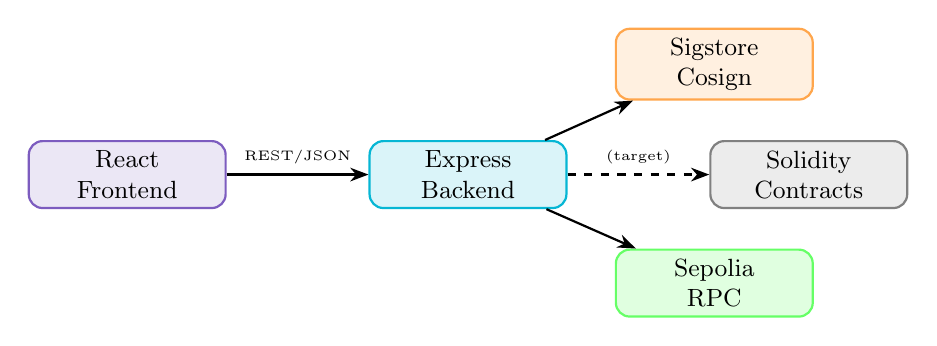
\begin{tikzpicture}[
  box/.style={rectangle,rounded corners=5pt,minimum width=2.5cm,minimum height=0.85cm,
              draw,thick,align=center,font=\small},
  arr/.style={-Stealth,thick},node distance=0.6cm and 1.8cm]
  \node[box,fill=accentpurple!15,draw=accentpurple](fe){React\\Frontend};
  \node[box,fill=accentcyan!15,draw=accentcyan,right=1.8cm of fe](be){Express\\Backend};
  \node[box,fill=green!12,draw=green!60,below right=0.5cm and 0.6cm of be](bc){Sepolia\\RPC};
  \node[box,fill=orange!12,draw=orange!70,above right=0.5cm and 0.6cm of be](sg){Sigstore\\Cosign};
  \node[box,fill=gray!15,draw=gray,right=1.8cm of be](ct){Solidity\\Contracts};
  \draw[arr](fe)--node[above,font=\tiny]{REST/JSON}(be);
  \draw[arr](be)--(bc); \draw[arr](be)--(sg);
  \draw[arr,dashed](be)--node[above,font=\tiny]{(target)}(ct);
\end{tikzpicture}
\caption{High-level architecture}
\end{figure}

\vspace{-0.5em}
\subsection{Directory Structure}
\vspace{-0.3em}
\begin{lstlisting}[language=bash]
verifiable-deployer/
├── backend/src/
│   ├── controllers/   # Express route handlers
│   ├── services/      # Artifact hashing, Sigstore, deployment validation
│   └── db/            # In-memory store (AuditApproval[], Deployment[])
├── frontend/src/
│   ├── components/    # Layout, glassmorphism cards, Iridescence WebGL
│   ├── pages/         # Dashboard, Verify, Register, Deployments, Audit, Artifact
│   └── api.ts         # Typed fetch client
└── contracts/
    ├── AuditRegistry.sol
    └── DeploymentRegistry.sol
\end{lstlisting}

% ============================================================
\section{Verification Pipeline}
% ============================================================

\begin{figure}[H]
\centering
\begin{tikzpicture}[
  step/.style={rectangle,rounded corners=6pt,minimum width=2.6cm,minimum height=1cm,
               draw=accentcyan,fill=accentcyan!10,align=center,font=\small\bfseries},
  arr/.style={-Stealth,thick,color=accentcyan},node distance=0.6cm]
  \node[step](s1){Step 1\\Artifact Hash};
  \node[step,right=0.6cm of s1](s2){Step 2\\Audit Approval};
  \node[step,right=0.6cm of s2](s3){Step 3\\Sigstore\\Verify};
  \node[step,right=0.6cm of s3](s4){Step 4\\Bytecode\\Match};
  \node[rectangle,rounded corners=6pt,minimum width=2cm,minimum height=1cm,
        draw=green!60,fill=green!10,right=0.6cm of s4,align=center,
        font=\small\bfseries,text=green!60!black](ok){TRUSTED\\Record};
  \draw[arr](s1)--(s2);\draw[arr](s2)--(s3);\draw[arr](s3)--(s4);\draw[arr](s4)--(ok);
\end{tikzpicture}
\caption{Four-step fail-closed verification pipeline}
\end{figure}

\subsection{Step 1 — Artifact Hashing}
The backend reads the Hardhat/Foundry JSON artifact and computes three SHA-256 digests:
the raw file bytes (\textit{artifact hash}), \texttt{bytecode.object} (\textit{creation
bytecode hash}), and \texttt{deployedBytecode.object} (\textit{runtime bytecode hash}).

\subsection{Step 2 — Audit Approval}
Before registration, an auditor must have pre-approved the exact
\texttt{(artifactHash,~version)} pair via \texttt{POST /api/audit/approve}.
The check is: $\exists\,a \in \text{audits} : a.\text{hash} = H \wedge a.\text{version} = v$.

\subsection{Step 3 — Sigstore / Cosign Verification}
The backend shells out to \texttt{cosign verify-blob}, passing the artifact path, bundle
path, trusted OIDC issuer, and signer identity. Keyless signing relies on
\textbf{Fulcio} (short-lived X.509 cert bound to OIDC identity) and
\textbf{Rekor} (append-only transparency log). Failure causes include: \texttt{cosign}
absent from PATH, missing bundle, or unconfigured policy environment variables.

\subsection{Step 4 — On-Chain Bytecode Match}
Using \texttt{viem}, the backend calls \texttt{eth\_getCode} on the given Sepolia address
and verifies:
\[
\text{SHA-256}\!\left(\texttt{eth\_getCode}(\text{address})\right) \stackrel{?}{=}
\text{SHA-256}\!\left(\texttt{deployedBytecode.object}\right)
\]
A mismatch means a different contract is at that address than what was compiled and approved.

% ============================================================
\section{Backend API}
% ============================================================

\begin{table}[H]
\centering\small
\caption{REST API endpoints}
\begin{tabularx}{\textwidth}{llX}
\toprule
\textbf{Method} & \textbf{Path} & \textbf{Description}\\
\midrule
POST & \texttt{/api/artifacts/hash}        & Compute SHA-256 hashes of a compiled artifact\\
POST & \texttt{/api/audit/approve}         & Record auditor approval for (hash, version)\\
POST & \texttt{/api/sigstore/verify}       & Standalone Cosign bundle verification\\
POST & \texttt{/api/deploy/verify}         & Full pipeline — verify only, no persistence\\
POST & \texttt{/api/deployments}           & Full pipeline — verify and register if trusted\\
GET  & \texttt{/api/deployments}           & List all registered deployments\\
GET  & \texttt{/api/deployments/:address}  & Lookup deployment by contract address\\
\bottomrule
\end{tabularx}
\end{table}

The response from \texttt{POST /api/deployments} on success is a \texttt{Deployment}
object with fields: \texttt{contractAddress}, \texttt{chainId}, \texttt{artifactHash},
\texttt{runtimeBytecodeHash}, \texttt{version}, \texttt{signerIdentity},
\texttt{auditApproved}, \texttt{sigstoreVerified}, \texttt{bytecodeVerified},
\texttt{status} (\texttt{"TRUSTED"} or \texttt{"REJECTED"}), and \texttt{reasons[]}.

% ============================================================
\section{Smart Contracts}
% ============================================================

\subsection{AuditRegistry}
Stores auditor approvals on-chain using OpenZeppelin \texttt{AccessControl}.
Key mapping: \texttt{approvals[artifactHash][version] => Approval}.
Functions: \texttt{approveArtifact} (AUDITOR\_ROLE), \texttt{revokeApproval} (ADMIN\_ROLE),
\texttt{isApproved} (view).

\subsection{DeploymentRegistry}
Stores deployment records keyed by \texttt{keccak256(contractAddress, chainId)}.
References \texttt{AuditRegistry} via \texttt{IAuditRegistry}. Each record mirrors the
backend \texttt{Deployment} struct with additional fields \texttt{artifactURI},
\texttt{auditor} address, and individual boolean flags settable by ADMIN\_ROLE.

\begin{lstlisting}[language=Solidity,caption={DeploymentRegistry key function}]
function _deploymentKey(address _addr, uint256 _chainId)
    internal pure returns (bytes32) {
    return keccak256(abi.encodePacked(_addr, _chainId));
}
\end{lstlisting}

% ============================================================
\section{Frontend \& UI}
% ============================================================

\subsection{Pages}
Dashboard (stats + pipeline diagram), Verify (4-check form), Register (verify + persist),
Deployments (searchable list + detail view), Audit Approve, and Artifact Hash.

\subsection{Design — Glassmorphism over Iridescence}
A full-viewport \textbf{WebGL Iridescence} shader (\texttt{ogl} library, colour
\texttt{\#06b6d4}) renders shifting cyan/teal waves as the background. Sidebar, topbar,
and cards float over it as \textbf{dark glass panels} —
\texttt{rgba(4,2,14,0.78)} background with \texttt{backdrop-filter:~blur(20px)~saturate(200\%)}
— matching the frosted-glass terminal aesthetic. Purple gradient
(\texttt{\#7c5cbf}→\texttt{\#a78bfa}) is used for active navigation and primary actions;
green (\texttt{\#4ce4a2}) for trusted status; red (\texttt{\#f06292}) for rejected.

\begin{table}[H]
\centering\small
\caption{Technology stack summary}
\begin{tabular}{lll}
\toprule
\textbf{Layer} & \textbf{Technology} & \textbf{Version}\\
\midrule
Backend runtime   & Node.js + Express    & v20 / v5\\
Backend language  & TypeScript           & 5\\
Ethereum client   & viem                 & v2\\
Keyless signing   & Cosign / Sigstore    & latest\\
Frontend          & React + Vite         & 19 / 7\\
Styling           & Tailwind CSS         & v3\\
WebGL background  & ogl (Iridescence)    & latest\\
Contracts         & Solidity + OpenZeppelin & \^{}0.8.24\\
\bottomrule
\end{tabular}
\end{table}

% ============================================================
\section{Security Analysis \& Limitations}
% ============================================================

\subsection{Threat Mitigations}
\begin{itemize}[leftmargin=1.5em,itemsep=1pt]
  \item \textbf{Tampered artifact} — artifact hash mismatch detected in Step~1.
  \item \textbf{Unaudited deployment} — audit approval check rejects unknown hashes (Step~2).
  \item \textbf{Supply chain / wrong identity} — Cosign verifies OIDC issuer and signer (Step~3).
  \item \textbf{Bytecode substitution} — \texttt{eth\_getCode} comparison detects mismatch (Step~4).
  \item \textbf{Duplicate registration} — 409 conflict on \texttt{(address, chainId)} uniqueness.
\end{itemize}

\subsection{Known Limitations}
\begin{itemize}[leftmargin=1.5em,itemsep=1pt]
  \item In-memory store resets on restart — replace with a persistent database for production.
  \item No API authentication or rate limiting — all endpoints are publicly accessible.
  \item \texttt{cosign} must be installed in PATH; absence fails all signature checks.
  \item Chain ID is hardcoded to Sepolia (11155111).
  \item Solidity contracts are not yet wired to the backend (in-memory store used instead).
\end{itemize}

% ============================================================
\section{Conclusion}
% ============================================================

The Verifiable Smart Contract Deployer demonstrates that a rigorous cryptographic
chain of custody for smart contract deployments can be built using existing open-source
tooling. By combining SHA-256 artifact hashing, on-chain auditor approvals, keyless
Sigstore signing, and live bytecode verification, the system creates a four-factor proof
that a deployed contract matches its approved, signed build artifact. The fail-closed
architecture ensures that partial failures are never silently ignored, making this a
practical reference implementation for teams seeking to raise the security bar on their
deployment pipelines.

% ── References ───────────────────────────────────────────────
\begin{thebibliography}{6}\small
\bibitem{sigstore} Sigstore Project. \textit{Sigstore: A New Standard for Signing Software}. \url{https://www.sigstore.dev}, 2024.
\bibitem{cosign} Sigstore. \textit{Cosign: Container Signing and Verification}. \url{https://github.com/sigstore/cosign}, 2024.
\bibitem{oz} OpenZeppelin. \textit{OpenZeppelin Contracts}. \url{https://docs.openzeppelin.com/contracts}, 2024.
\bibitem{viem} wevm. \textit{viem: TypeScript Interface for Ethereum}. \url{https://viem.sh}, 2024.
\bibitem{sepolia} Ethereum Foundation. \textit{Sepolia Testnet}. \url{https://sepolia.dev}, 2024.
\bibitem{ethereum} Buterin, V. \textit{Ethereum Whitepaper}. \url{https://ethereum.org/en/whitepaper}, 2014.
\end{thebibliography}

\end{document}
